%%%%%%%%%%%%%%%%%%%%%%%%%%%%%%%%%%%%%%%%%%%%%%%%%%%%%%%%%%%%%%%%%%%%%%%%%%%%%%%%%%%%
%Do not alter this block of commands.  If you're proficient at LaTeX, you may include additional packages, create macros, etc. immediately below this block of commands, but make sure to NOT alter the header, margin, and comment settings here. 
\documentclass[12pt]{article}
\usepackage{amsmath,amsthm,amssymb,amsfonts, enumitem, fancyhdr, color, comment, graphicx, environ, algorithm, algpseudocode}




%\pagestyle{fancy}
%\setlength{\headheight}{65pt}
\newenvironment{problem}[2][Problem]{\begin{trivlist}
\item[\hskip \labelsep {\bfseries #1}\hskip \labelsep {\bfseries #2.}]}{\end{trivlist}}
\newenvironment{sol}
    {\emph{Solution:}
    }
    {
    \qed
    }
\specialcomment{com}{ \color{blue} \textbf{Comment:} }{\color{black}} %for instructor comments while grading
\NewEnviron{probscore}{\marginpar{ \color{blue} \tiny Problem Score: \BODY \color{black} }}
%%%%%%%%%%%%%%%%%%%%%%%%%%%%%%%%%%%%%%%%%%%%%%%%%%%%%%%%%%%%%%%%%%%%%%%%%%%%%%%%%


%%%%%%%%%%%%%%%%%%%%%%%%%%%%%%%%%%%%%%
%Do not alter this block.
\begin{document}
%%%%%%%%%%%%%%%%%%%%%%%%%%%%%%%%%%%%%%

\title{Homework \#10 \\ CPSC 250 \\ (Extra Credit)\\ Due: Friday, December 6th \\ Tanner Hammond}
\date{}

\maketitle

\begin{enumerate}
\item (20)
Consider the following ``greedy” strategy for solving the rod cutting problem.
Define the density of a rod of length i to be $p_i/i$, that is, its value per inch.
The greedy strategy for a rod of length $n$ cuts off a first piece of length i, where
$1 \leq i \leq n$, has maximum density. It then continues by applying the greedy strategy to 
the remaining piece of length $n-i$.

\begin{enumerate}
\item Use the rod cutting problem of Figure 15.1 (figure included at the end.) to prove that 
this ``greedy" strategy isn't optimal. Do this by showing an $n \in [1,10]$ for which the output 
of this algorithm isn't optimal. Show your work.
\newline Answer: There are several situations where the strategy isn't optimal. Some lengths are better to not be cut such as a rod of length 10 or 6. If you do a rod of length 10, the best profit you can get is 1 + 9 which is 25. For 6 it would be 14 If you didn't cut them at all, 10 would be 30 and 6 would be 17.
\item What is the time complexity of this algorithm? Justify your answer. \newline Answer: The time complexity is $nlgn$, because you have a for loop with an algorithm that takes lgn time.
\end{enumerate}

\item (10)
Use mathematical induction to prove that $T(n) = 2^n$, where
$T(n) = 1 + \Sigma_{i = 0}^{n-1} T(i).$ Recall that the sum over an empty range is 0.
\begin{itemize}
\item Bases case: The base case of this mathematical induction is where the range is 0. This makes the two equations both 1. $2^0$ = 1 and 1 + 0 = 1.
\item Inductive step: Hence the base case holds true, assume it's true for n > 0. T(n+1) = 1 + $\Sigma_{j=0}^{n}T$(j) = 1 + ($1+2^1 + 2^2+ ... + 2^n$) = 1 + (1 - $2^{n+1}$)/(1-2) = $2^{n+1}$
\item Conclusion: Thus it holds true for all cases.
\end{itemize}

\item (30) The Fibonacci numbers are defined by recurrence following recurrence.
\[
 F(n) = \begin{cases}
         0 &n  = 0\\
         1 &n  = 1\\
         F(n-1) + F(n-2) &n > 1
        \end{cases}
\]

\begin{enumerate}
\item Give a $O(n)$-time dynamic-programming algorithm to compute the $n$th Fibonacci number.

\begin{algorithm}[H]
 \begin{algorithmic}[1]
 \Procedure{F($n$)}{}
 \State int f[n+2]
 \State int i
 \State f[0] = 0
 \State f[1] = 1
 \State for(i=2; i \textless= n; i++)
 \State \indent f[i] = f[i-1] + f[i-2]
 \State return f[n]
 \EndProcedure
\end{algorithmic}
\end{algorithm}

\item Draw the subproblem graph (You can do it by hand on your printout, just make sure it's 
drawn NEATLY).
\newline Answer:

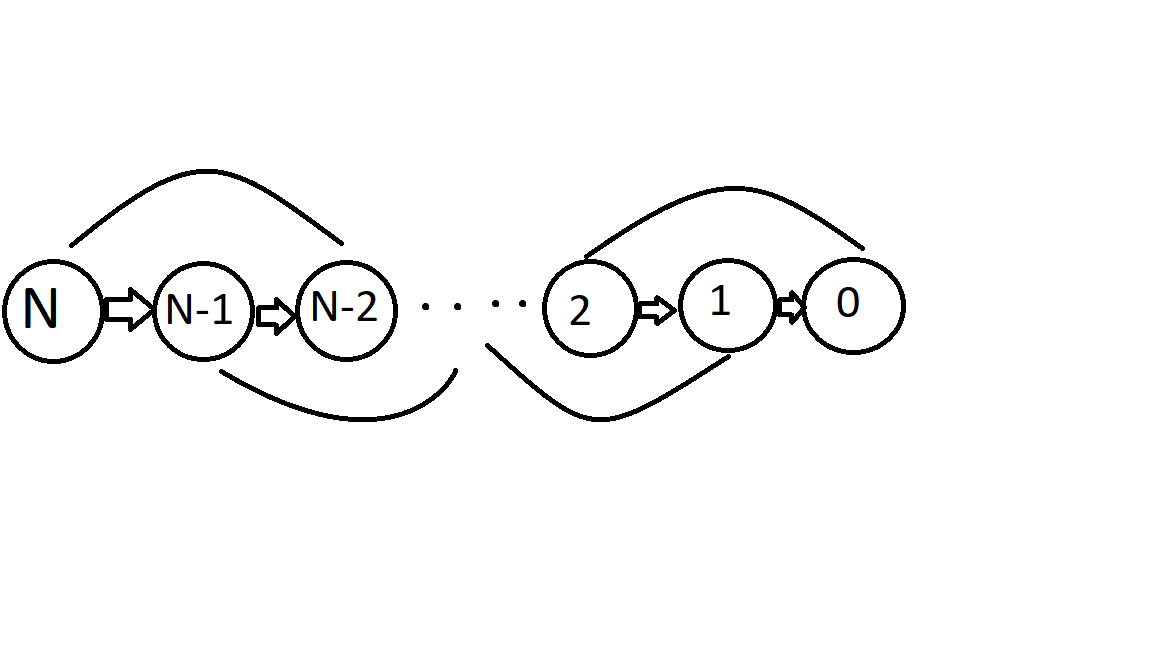
\includegraphics[scale = 0.25]{Fibon}

\item How many vertices and edges are in the graph? Show your work.
\newline Answer: (n+1) + n + n-1 + n-2 + .... +1 + 0. Vertices and edges will be ((n+1)(n+2))/2
\end{enumerate}

\item (10) Show the red-black trees that result after:
\begin{enumerate}
\item  successively inserting the keys 41, 38, 
31,12, 19, 8 into an initially empty red-black tree.

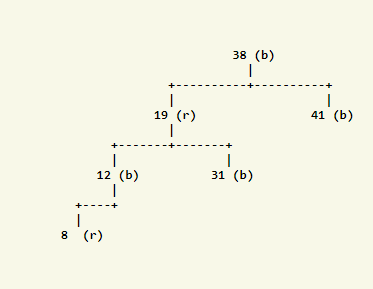
\includegraphics[scale = 0.75]{RBT1}

\item removing the root.
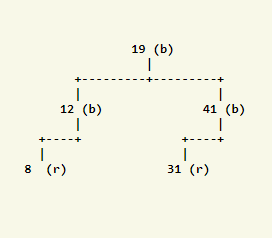
\includegraphics[scale = 0.75]{RBT2}
\end{enumerate}

\item (10) Suppose that the black-height of each of the subtrees
$\alpha, \beta, \gamma, \delta,\epsilon$ in Figures 13.5
and 13.6 is $k$. Label each node in each figure with its black-height to verify that
the indicated transformation preserves property 5.

\end{enumerate}

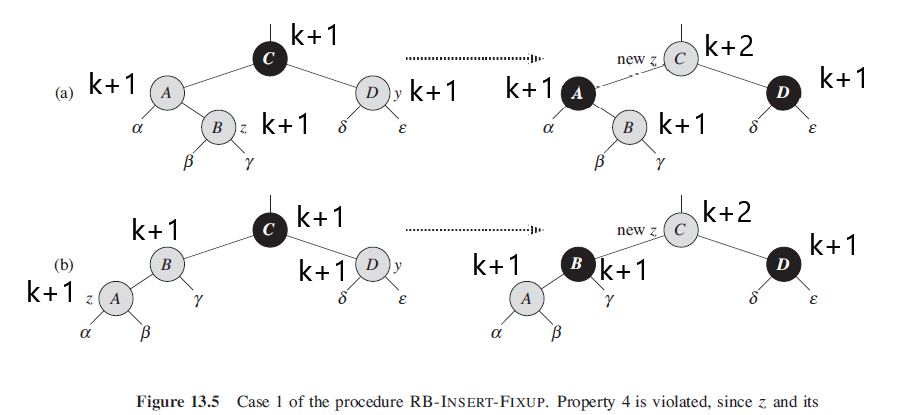
\includegraphics[scale=0.55]{fig_13_5}
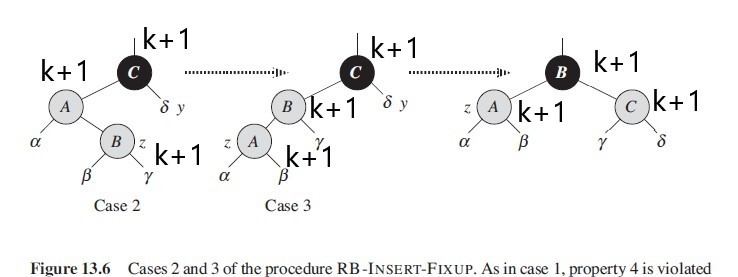
\includegraphics[scale=0.75]{fig_13_6}


%Copy the following block of text for each problem in the assignment.
%\begin{problem}{1}
%\end{problem}
%%%%%%%%%%%%%%%%%%%%%%%%%%%%%%%%%%%%%%%%
%Do not alter anything below this line.
\end{document}